\documentclass[conference,a4paper]{IEEEtran}
\usepackage{cite}
\usepackage{amsmath,amssymb}
\usepackage{graphicx}
\graphicspath{{assets/}{./}}
\usepackage{booktabs}
\usepackage{balance}
\usepackage{tikz}
\usetikzlibrary{arrows.meta,positioning}
\usepackage[hidelinks]{hyperref}

\begin{document}
\title{Outflow-Tract Arrhythmia Localization Using a Compact 1D CNN Ensemble with a Web-Based IoT Gateway}
\author{
\IEEEauthorblockN{Daniandra Prayudisty Ilham}
\IEEEauthorblockA{\textit{Informatics, School of Computing}\\
\textit{Telkom University}\\Bandung 40257, Indonesia\\
daniandraaa@student.telkomuniversity.ac.id}
\and
\IEEEauthorblockN{Satria Mandala}
\IEEEauthorblockA{\textit{Humic Engineering, School of Computing}\\
\textit{Telkom University}\\Bandung 40257, Indonesia\\
satriamandala@telkomuniversity.ac.id}}
\maketitle

\begin{abstract}
An Internet of Things (IoT) service that localizes ventricular arrhythmia origins from 12-lead electrocardiograms (ECGs) must deliver the same decision that was validated offline, within a predictable processing time. This study develops a compact one-dimensional convolutional neural network (1D CNN) ensemble that classifies left versus right ventricular outflow-tract (LVOT/RVOT) origin at record level, and deploys it behind an HTTP/JSON gateway with a browser dashboard. A Random Forest (RF) using 132 morphology and RR-interval features and three established ECG criteria serve as comparators. On 230 development patients, five patient-level folds with three initialization seeds gave a macro-F1 of 0.903 for the selected CNN and 0.775 for RF, with LVOT sensitivities of 0.859 and 0.620. All ten evaluated CNN training configurations, including a pre-specified configuration without generative augmentation (macro-F1 0.891), exceeded RF. A patient-level bootstrap of out-of-fold predictions gave a CNN--RF macro-F1 difference of 0.120 (95\% CI 0.056--0.186). On a 59-patient historical hold-out, the five-model ensembles reached macro-F1 of 0.828 and 0.721, and ROC AUC of 0.941 and 0.741. Gateway replay preserved all 59 offline class predictions. After the source of a CNN latency tail was identified and removed, repeated measurements gave CNN and RF pipeline medians of 57.8 and 104.2~ms and 95th percentiles of 109.6 and 132.8~ms per record. Physical-device acquisition and external validation remain future work.
\end{abstract}
\begin{IEEEkeywords}
Internet of Things, 12-lead ECG, ventricular arrhythmia, outflow-tract localization, convolutional neural network, Random Forest
\end{IEEEkeywords}

\section{Introduction}
Idiopathic premature ventricular contractions (PVCs) and ventricular tachycardia (VT) most often arise from the left or right ventricular outflow tract (LVOT or RVOT). Predicting the side before catheter ablation helps plan vascular access and procedure time, but manual criteria such as the V2 transition ratio~\cite{betensky2011} and V2S/V3R index~\cite{yoshida2014} depend on careful reading of precordial morphology. The public Ningbo database provides 12-lead PVC/VT recordings labelled with successful ablation sites~\cite{zheng2020}, enabling data-driven localization.

Connected ECG recorders increasingly send digital 12-lead records to remote services rather than printing them for local reading. For such an IoT service, an accurate model is necessary but not sufficient. The service must (i) apply exactly the preprocessing used during model development to records that arrive in chunks over a network, (ii) return the same decision as the validated offline model, and (iii) do so within a bounded processing time on modest hardware. Most ECG learning studies report accuracy offline~\cite{hannun2019,ribeiro2020,zheng2021} and leave these deployment properties unmeasured.

This paper addresses localization and deployment together. Its contributions are:
\begin{itemize}
\item A compact CNN pipeline for record-level LVOT/RVOT localization that, under matched patient partitions, exceeds a morphology-based RF and three established ECG criteria in macro-F1 and LVOT sensitivity. We show that this advantage holds for every evaluated CNN training configuration and does not depend on generative augmentation.
\item An IoT gateway protocol (session declaration, sequenced chunks, completeness checks, server-side canonical preprocessing) with a verification procedure showing that gateway outputs reproduce offline model probabilities record by record.
\item A repeated latency benchmark that separates model inference from pipeline and gateway time. It identifies a batch-size-dependent CPU convolution slowdown as the cause of CNN tail latency, and shows that fixed 8-window inference batches remove it without changing any prediction.
\end{itemize}
The system performs post-acquisition localization of complete records. Experiments use real public-dataset recordings injected at the gateway; live physical-device acquisition is outside the evaluated scope.

\section{Related Work}
Conventional criteria express relationships among precordial morphologies: the transition zone, the V2 transition ratio~\cite{betensky2011}, and the V2S/V3R index~\cite{yoshida2014}. Zheng \emph{et al.} released the 334-patient database used here~\cite{zheng2020} and classified left/right origin with engineered features and machine learning~\cite{zheng2021}. Their representation differs from our 132-feature RF, which is therefore a local comparator with stated settings rather than a reproduction of their classifier.

Deep networks learn ECG representations directly for rhythm classification~\cite{hannun2019} and 12-lead diagnosis~\cite{ribeiro2020}, but those targets and cohorts differ from anatomical origin localization. On the IoT side, Ardian and Mandala~\cite{ardian2025} coupled a modified Transformer decoder and a conditional ECG-GAN with a web application for beat classification. The present work differs in output (record-level anatomical origin rather than beat class) and in evaluation: we verify decision preservation through the gateway and characterise latency tails with repeated measurements, rather than reporting offline accuracy alone.

\section{Methodology}
\subsection{System Overview}
Fig.~\ref{fig:system} shows the acquisition-to-user path. A complete 12-lead record enters through the HTTP gateway, receives canonical preprocessing on the server, and is classified by the CNN ensemble; the browser presents the LVOT/RVOT output and stage timing. The RF branch is a separately timed comparator. A physical ECG recorder is the intended upstream source (dashed); the experiments inject real public-dataset recordings at the gateway and evaluate the solid paths.

\begin{figure*}[t]
\centering
\resizebox{\textwidth}{!}{%
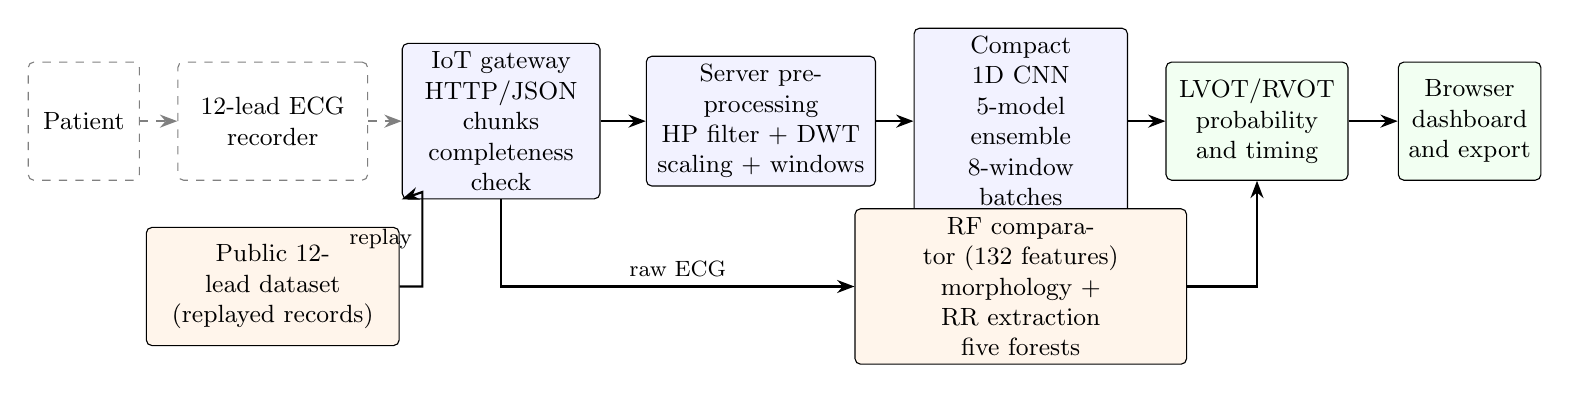
\begin{tikzpicture}[font=\small,
 box/.style={draw,rounded corners=2pt,align=center,minimum height=15mm,inner sep=3pt},
 arr/.style={-{Stealth[length=2.2mm]},thick},
 target/.style={arr,dashed,gray}]
\node[box,text width=12mm,dashed,draw=gray] (patient) at (0,0) {Patient};
\node[box,text width=22mm,dashed,draw=gray] (device) at (2.4,0) {12-lead ECG\\recorder};
\node[box,text width=23mm,fill=blue!5] (gateway) at (5.3,0) {IoT gateway\\HTTP/JSON chunks\\completeness check};
\node[box,text width=27mm,fill=blue!5] (pre) at (8.6,0) {Server preprocessing\\HP filter + DWT\\scaling + windows};
\node[box,text width=25mm,fill=blue!5] (cnn) at (11.9,0) {Compact 1D CNN\\5-model ensemble\\8-window batches};
\node[box,text width=21mm,fill=green!5] (output) at (14.9,0) {LVOT/RVOT\\probability\\and timing};
\node[box,text width=16mm,fill=green!5] (user) at (17.6,0) {Browser\\dashboard\\and export};
\node[box,text width=30mm,fill=orange!8] (dataset) at (2.4,-2.1) {Public 12-lead dataset\\(replayed records)};
\node[box,text width=40mm,fill=orange!8] (rf) at (11.9,-2.1) {RF comparator (132 features)\\morphology + RR extraction\\five forests};
\draw[target] (patient)--(device);
\draw[target] (device)--(gateway);
\draw[arr] (gateway)--(pre);
\draw[arr] (pre)--(cnn);
\draw[arr] (cnn)--(output);
\draw[arr] (output)--(user);
\draw[arr] (dataset.east)--(4.3,-2.1)--node[left,font=\footnotesize]{replay}(4.3,-.9)--(gateway.south west);
\draw[arr] (gateway.south)--(5.3,-2.1)--node[above,font=\footnotesize]{raw ECG}(rf.west);
\draw[arr] (rf.east)-|(output.south);
\end{tikzpicture}}
\caption{Acquisition-to-user architecture. Solid paths are implemented and evaluated; dashed paths (physical recorder) are the intended source but were not evaluated. The RF branch receives the raw record and performs its own feature processing.}
\label{fig:system}
\end{figure*}

\subsection{Dataset, Cohort Definition, and Class Imbalance}
The Ningbo resource contains 334 subjects recorded at 2000~Hz~\cite{zheng2020}. This study uses a cohort frozen in earlier work on the same models: five Summit records and 40 records without a \texttt{Sublocation} entry were excluded. All 334 subjects have a coarse left/right label, so the 40 exclusions are a cohort-definition choice, not missing outcomes. The frozen cohort was retained so that the fold assignment, historical hold-out, and deployed model artifacts remain identical across all analyses reported here; it also allows per-sublocation error analysis. Because the excluded records still have binary labels, their omission may make the cohort less representative; we discuss this in Section~\ref{sec:limits}.

The 289 included patients comprise 71 LVOT and 218 RVOT cases (286 PVC and 3 VT records). Table~\ref{tab:cohort} gives the 230-patient development and 59-patient historical hold-out partitions; all splits are by patient. The 1:3 imbalance is handled in four ways: stratified folds, a class-weighted patient loss for the CNN, balanced class weights for RF, and reporting macro-F1, balanced accuracy, and LVOT sensitivity rather than accuracy alone. The three VT records are too few for separate analysis, so results describe a predominantly PVC population.

\begin{table}[t]
\caption{Frozen cohort and partition counts.}
\label{tab:cohort}\centering
\begin{tabular}{lrrr}\toprule
Partition & LVOT & RVOT & Total\\\midrule
Development & 57 & 173 & 230\\
Historical hold-out & 14 & 45 & 59\\\midrule
Included cohort & 71 & 218 & 289\\\bottomrule
\end{tabular}
\end{table}

\subsection{ECG Preprocessing}
Leads are ordered I, II, III, aVR, aVL, aVF, V1--V6 at native amplitude and sampling rate. The complete record is high-pass filtered (fourth-order Butterworth, 0.5~Hz, forward--backward) and denoised with a level-five coif5 wavelet transform using SURE soft thresholds~\cite{donoho1995}. The denoised signal is cut into complete 5000-point windows (2.5~s) with a 2500-point step, and each lead is standardized with statistics from training patients only. Forward--backward filtering and record-level wavelet thresholds are noncausal: they need the whole record. The deployed service therefore performs \emph{post-acquisition} localization. It returns one decision after the record is complete, not continuous beat-by-beat output. This suits the intended use, a pre-procedural origin estimate from a resting 12-lead recording, but would need causal filters for continuous monitoring.

\subsection{Compact CNN and Training}
Each CNN has four convolutional blocks with 32, 64, 128, and 256 channels and kernel lengths 7, 5, 3, and 3. Each block applies same-padded convolution, batch normalization, ReLU, and max pooling by two. Global temporal averaging feeds layer normalization, a 256-to-128 linear layer, ReLU, dropout 0.3, and a two-output layer. Each model has 170,914 trainable parameters. With window probabilities $p_{s,w}(c)$ from seed $s$ and window $w$, and $W_i$ complete windows in patient $i$, the single-model and ensemble probabilities are
\begin{equation}
\bar p_{i,s}(c)=\frac{1}{W_i}\sum_{w=1}^{W_i}p_{s,w}(c),\qquad
\hat p_i(c)=\frac{1}{5}\sum_{s}\bar p_{i,s}(c).
\label{eq:pool}
\end{equation}
RVOT is assigned when $\hat p_i(\mathrm{RVOT})>0.5$.

Training samples bags of up to four windows per patient and applies a class-weighted negative log-likelihood after mean pooling. The bag size is a memory and diversity budget: random four-window draws expose the model to different parts of each recording across epochs. Because pooling is a mean of window probabilities, the training bag and the inference record estimate the same patient-level quantity. Inference averages all complete windows, which uses all available signal and reduces the variance of that estimate. A conditional GAN~\cite{mirza2014}, fitted only to the training patients of each fold, can replace one window of a four-window bag with a class-matched synthetic window. Validation, hold-out, and gateway inference use only real ECG.

AdamW (weight decay $10^{-4}$), cosine decay to $10^{-6}$, gradient clipping at 1.0, and early stopping with patience 15 on validation macro-F1 were used throughout. Ten training configurations were evaluated: nine GAN-augmented configurations crossing learning rates $\{10^{-4},5\times10^{-4},10^{-3}\}$ with window budgets $\{16,32,64\}$ (G01--G09), and a configuration without augmentation (learning rate $10^{-3}$, budget 32) that had been specified in advance as the reference. G04 ($5\times10^{-4}$, 16, GAN) had the highest mean CV macro-F1 and was deployed. Five final CNNs (seeds 42--46) were fitted on all 230 development patients for 16 epochs.

\subsection{Comparators}
\emph{Random Forest.} The RF~\cite{breiman2001} uses 132 features from the raw recording: per-lead QRS width, relative R and S amplitudes, R fraction, and signed QRS area; global QRS span, precordial transition, V2S/V3R; and three RR measures, each summarized by the median and interquartile range over detected beats. Missing values are median-imputed from training patients. Each forest has 500 trees, balanced class weights, and default scikit-learn settings otherwise; the RF was not tuned. It uses the same folds and seeds as the CNN, and deployment averages five forests.

\emph{Established ECG criteria.} Three published rules were computed without training on the same patients: transition zone (LVOT if $\le$V2, RVOT if $\ge$V4, indeterminate at V3), V2S/V3R index ($\le1.5$ indicates LVOT)~\cite{yoshida2014}, and V2 transition ratio ($\ge0.6$ indicates LVOT)~\cite{betensky2011}. Records where a criterion cannot be measured are assigned RVOT, the majority class.

\subsection{Evaluation Protocol}
Five fixed stratified folds on the 230 development patients were evaluated with seeds 42--44, giving 15 paired fits per model. These fits share patients and folds and are not independent. We therefore report uncertainty at two levels. Fit-level paired differences use the corrected resampled $t$ statistic of Nadeau and Bengio~\cite{nadeau2003}. For patient-level uncertainty, the three seed predictions of each out-of-fold patient are averaged to give one probability per patient (230 in total). A class-stratified bootstrap over patients (5000 resamples) then gives intervals for the CNN--RF difference. Because G04 was chosen on the same folds, the CV estimate for G04 is optimistic. We quantify this by reporting all ten configurations, including the reference without augmentation. Hold-out ensemble differences use the same patient bootstrap and an exact McNemar test~\cite{mcnemar1947}. The hold-out had been inspected in earlier exploratory work and is secondary evidence, not an untouched test set.

\subsection{Web and IoT Deployment}
The service uses a Python HTTP server, PyTorch CNN inference, a scikit-learn RF comparator, and a browser dashboard. A client opens a session that declares sampling rate, lead order, amplitude unit, and expected length. It then sends sequenced JSON chunks (at most 8000 time points each) with sample offsets. Identical retransmissions are accepted once; gaps, conflicts, and inconsistent offsets are rejected. Finalization checks completeness before preprocessing and inference. CNN checkpoints and the scaler are verified against SHA-256 hashes; the deployed identity is \texttt{154da12ade375dff}. The CNN processes windows in fixed batches of 8 (Section~\ref{sec:latency}).

\emph{Consistency test.} All 59 hold-out records were sent through the gateway in 1000-point chunks (0.5~s of signal each) without delay. Five records were also replayed at acquisition pace (2000 points/s). Gateway probabilities were compared with offline probabilities.

\emph{Latency benchmark.} Each of the 59 hold-out records was processed ten times after one warm-up, alternating CNN-first and RF-first order. Runs used 1 and 4 PyTorch threads, giving 1180 timed trials per thread setting. CNN pipeline time is preprocessing plus five-model inference; RF pipeline time is feature extraction plus five-forest inference. File I/O, network, browser, and model loading are excluded and reported separately from gateway timing. All runs used one Apple Silicon (arm64) workstation, macOS 26.2, PyTorch 2.12.0, CPU inference, and one job per forest.

\section{Results}
\subsection{Development Cross-Validation}
Table~\ref{tab:cv} compares the deployed CNN configuration, the reference CNN without augmentation, RF, and the three ECG criteria on the 230 development patients. The selected CNN reaches macro-F1 0.903 compared with 0.775 for RF, a paired difference of 0.128 (corrected 95\% CI 0.025--0.231, $p=0.019$). The CNN has higher macro-F1 in 13 of 15 fits and ties in two. The largest gain is in the minority class: LVOT sensitivity is 0.859 for CNN and 0.620 for RF. RVOT sensitivity is 0.950 and 0.915. The CNN is also more stable across fits (SD 0.028 versus 0.081). The best ECG criterion (transition zone) reaches macro-F1 0.732; V2S/V3R gives 0.711 and the V2 transition ratio 0.500.

\begin{table}[t]
\caption{Development CV on 230 patients (mean $\pm$ SD over 15 fold/seed fits; ECG criteria are deterministic). BA: balanced accuracy; Sens.~L: LVOT sensitivity.}
\label{tab:cv}\centering\small
\setlength{\tabcolsep}{3pt}
\resizebox{\columnwidth}{!}{%
\begin{tabular}{lcccc}\toprule
Method & Macro-F1 & AUC & BA & Sens.~L\\\midrule
CNN, deployed (G04) & \textbf{.903}$\pm$.028 & \textbf{.935}$\pm$.026 & \textbf{.905}$\pm$.034 & \textbf{.859}$\pm$.078\\
CNN, no augmentation & .891$\pm$.031 & .931$\pm$.023 & .897$\pm$.021 & .859$\pm$.056\\
Random Forest & .775$\pm$.081 & .851$\pm$.077 & .767$\pm$.086 & .620$\pm$.174\\\midrule
Transition zone & .732 & .749 & .711 & .491\\
V2S/V3R index & .711 & .835 & .771 & .825\\
V2 transition ratio & .500 & .824 & .612 & .825\\\bottomrule
\end{tabular}}
\end{table}

\emph{Robustness to configuration selection.} Fig.~\ref{fig:configs} shows all ten CNN configurations. Mean macro-F1 ranges from 0.872 (G03) to 0.903 (G04), and every configuration exceeds RF in at least 12 of 15 paired fits. The best-minus-worst spread of 0.031 bounds how much selecting G04 on the same folds can inflate its estimate. That spread is about a quarter of the 0.128 CNN--RF difference. The reference configuration without augmentation, which was not selected, still exceeds RF by 0.116.

\begin{figure}[t]\centering
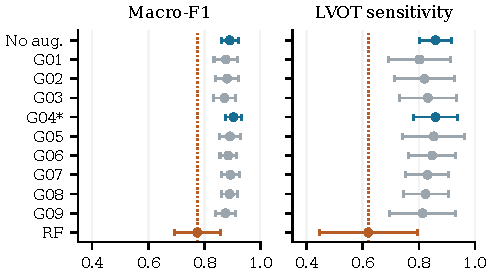
\includegraphics[width=\columnwidth]{cv_configurations.pdf}
\caption{Mean $\pm$ SD over 15 fold/seed fits for all ten CNN training configurations and RF (dotted line: RF mean). Blue: deployed G04 (*) and the pre-specified configuration without augmentation.}
\label{fig:configs}
\end{figure}

\emph{Patient-level uncertainty.} Using one out-of-fold probability per patient, the CNN reaches macro-F1 0.899 and AUC 0.946, against 0.779 and 0.842 for RF. The patient bootstrap gives a macro-F1 difference of 0.120 (95\% CI 0.056--0.186) and an AUC difference of 0.104 (0.031--0.183). For the no-augmentation CNN, the macro-F1 difference is 0.116 (0.049--0.184). Both intervals exclude zero.

\subsection{Contribution of GAN Augmentation}
G08 and the no-augmentation configuration share learning rate, window budget, architecture, folds, seeds, and epoch limit; they differ only in GAN augmentation. Their mean macro-F1 values are identical to three decimals (0.891 and 0.891); AUC is 0.931 for both. LVOT sensitivity is 0.824 with GAN and 0.859 without. At patient level the difference in macro-F1 is $-0.008$ (95\% CI $-0.038$ to 0.020). Conditional GAN augmentation therefore gave no measurable benefit here, and the CNN's advantage over RF does not come from augmentation. G04 remains the deployed model because it had the highest CV score. A deployment without the GAN would be simpler and is expected to perform similarly.

\subsection{Single Model Versus Ensemble}
Table~\ref{tab:ensemble} compares individual CNNs with seed ensembles under matched partitions. In CV, averaging three seeds per patient leaves macro-F1 essentially unchanged (0.899 versus a fit mean of 0.903) and raises AUC from 0.935 to 0.946. On the hold-out, the five-model ensemble improves macro-F1 from a single-model mean of 0.793 to 0.828 and AUC from 0.916 to 0.941. The ensemble also removes the seed-to-seed spread (SD 0.038) from the deployed decision. The cost is five times the parameters (854,570) and five forward passes. In the deployed service, those five passes take a median of 33.5~ms per record in total (Section~\ref{sec:latency}).

\begin{table}[t]
\caption{Individual CNN versus seed ensemble. Single-model values are means ($\pm$SD) over fits or seeds.}
\label{tab:ensemble}\centering\small
\setlength{\tabcolsep}{3pt}
\begin{tabular}{lcccc}\toprule
 & Macro-F1 & AUC & BA & Params\\\midrule
CV, single CNN & .903$\pm$.028 & .935 & .905 & 170,914\\
CV, 3-seed ensemble & .899 & .946 & .892 & 512,742\\
Hold-out, single CNN & .793$\pm$.038 & .916 & -- & 170,914\\
Hold-out, 5-seed ensemble & .828 & .941 & .862 & 854,570\\\bottomrule
\end{tabular}
\end{table}

\subsection{Historical Hold-Out}
Table~\ref{tab:holdout} and Fig.~\ref{fig:cm} summarize the deployed ensembles on 59 patients. The CNN correctly classifies 12 of 14 LVOT and 39 of 45 RVOT cases; RF classifies 7 LVOT and 41 RVOT cases correctly. The CNN gains in LVOT sensitivity (0.857 versus 0.500) at the cost of two RVOT cases. The AUC difference is 0.200 (95\% CI 0.067--0.349). The macro-F1 difference is 0.108 (95\% CI $-0.026$ to 0.257; McNemar $p=0.55$). With 14 LVOT patients and a previously inspected hold-out, this is supporting rather than confirmatory evidence. Hold-out macro-F1 (0.828) is lower than CV (0.903), consistent with the selection optimism discussed above.

\begin{table}[t]
\caption{Historical hold-out (59 patients, 14 LVOT): five-model ensembles.}
\label{tab:holdout}\centering\small
\begin{tabular}{lcc}\toprule
Metric & 1D CNN & Random Forest\\\midrule
Macro-F1 & \textbf{0.828} & 0.721\\
ROC AUC & \textbf{0.941} & 0.741\\
Accuracy & \textbf{0.864} & 0.814\\
Balanced accuracy & \textbf{0.862} & 0.706\\
LVOT sensitivity & \textbf{0.857} & 0.500\\
RVOT sensitivity & 0.867 & \textbf{0.911}\\\bottomrule
\end{tabular}
\end{table}
\begin{figure}[t]\centering
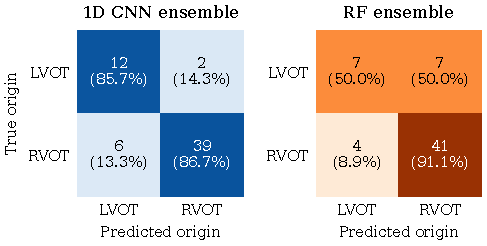
\includegraphics[width=\columnwidth]{holdout_confusion.pdf}
\caption{Historical hold-out confusion matrices with within-row percentages.}
\label{fig:cm}
\end{figure}

\subsection{Gateway Consistency and Application}
All 59 no-delay replays completed (record durations 5.1--25.0~s, median 12.9~s). Gateway and offline class predictions agree for 59/59 records for both models. The maximum absolute probability difference is $2.5\times10^{-7}$ for the CNN and zero for RF. All five acquisition-paced replays also preserve both predictions. This 100\% agreement measures implementation consistency: the gateway reproduces the validated model. Diagnostic accuracy remains that of Table~\ref{tab:holdout}. During paced replay, the median chunk round trip was 10.2~ms and the largest within-record chunk P95 was 51.6~ms, well below the 500~ms of signal each chunk represents. The transfer path therefore keeps pace with acquisition on the local link. Eleven automated tests exercise the real server and frozen models. They cover valid transfer, duplicate chunks, gap and conflict rejection, incomplete records, incompatible rate/lead/unit declarations, prediction parity, and result export; all pass.

Fig.~\ref{fig:webapp} shows the running dashboard for hold-out record ECG-231: the received 12 leads, completed transfer status, and an RVOT output (CNN probability 98.0\%, RF 82.2\%). The heart graphic is a schematic orientation cue, not a patient-specific map.

\begin{figure*}[t]
\centering
\begin{minipage}[t]{0.63\textwidth}
\centering
{\small\textbf{(a) Received 12-lead ECG and completed transfer}}\\[2pt]
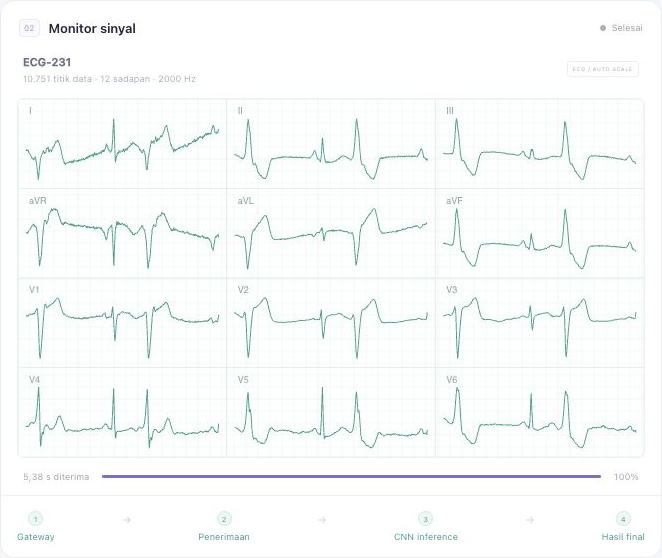
\includegraphics[width=\linewidth]{web_signal.png}\\[5pt]
{\small\textbf{(c) Development-CV summary panel}}\\[2pt]

\includegraphics[width=\linewidth]{web_cv_summary.png}
\end{minipage}\hfill
\begin{minipage}[t]{0.34\textwidth}
\centering
{\small\textbf{(b) Record-level localization output}}\\[2pt]
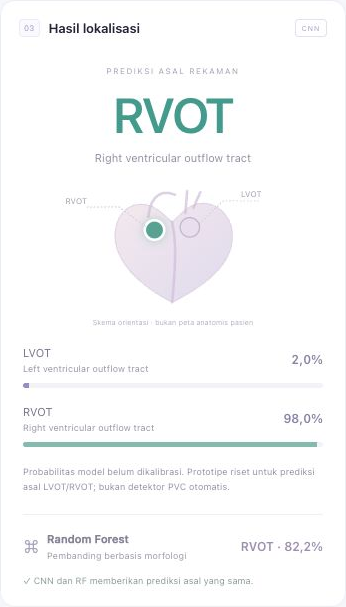
\includegraphics[width=\linewidth]{web_result.png}
\end{minipage}
\caption{Screenshots of the web application. (a) and (b): hold-out record ECG-231 (5.38~s, 12 leads, 2000~Hz) replayed at acquisition pace. (c): the separate CV summary panel. Interface values use Indonesian decimal commas.}
\label{fig:webapp}
\end{figure*}

\subsection{Processing Latency}
\label{sec:latency}
The first single-pass gateway measurement showed a lower CNN median but a long tail (P95 2370.6~ms against 254.4~ms for RF). Repeated measurements located the cause. The service ran CNN inference in batches of 16 windows, and on this PyTorch CPU build one-dimensional convolution becomes about 20 times slower once a batch holds 16 or more windows (one model: 15~ms for 15 windows, 371~ms for 16). Only records of at least 16 windows (about 21~s; 4 of 59 records) filled a full batch, which produced the tail. Processing windows in fixed batches of 8 removes the slowdown. Because the CNN evaluates each window independently, this does not change the output: class predictions agree in 1180/1180 trials, and the maximum probability difference is $2.5\times10^{-7}$.

\begin{table}[t]
\caption{Repeated latency benchmark: 59 records $\times$ 10 repeats (ms per record). Model computation only; I/O and network excluded.}
\label{tab:latency}\centering\small
\setlength{\tabcolsep}{4pt}
\resizebox{\columnwidth}{!}{%
\begin{tabular}{lrrrr}\toprule
 & \multicolumn{2}{c}{16-window batches} & \multicolumn{2}{c}{8-window batches}\\
Stage & Median & P95 & Median & P95\\\midrule
CNN inference, 5 models (4 thr.) & 39.4 & 2704.2 & 33.5 & 64.2\\
\textbf{CNN pipeline (4 threads)} & 64.4 & 2745.1 & \textbf{57.8} & \textbf{109.6}\\
CNN pipeline (1 thread) & 84.4 & 2822.9 & 83.2 & 162.6\\
RF features + 5 forests & 112.7 & 164.0 & 104.2 & 132.8\\\bottomrule
\end{tabular}}
\end{table}
\begin{figure}[t]\centering
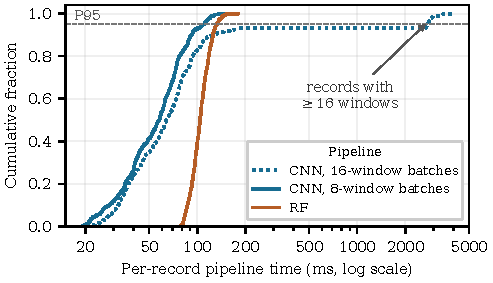
\includegraphics[width=\columnwidth]{latency_ecdf.pdf}
\caption{Empirical distributions of per-record pipeline time over 590 trials with four CNN threads. The dotted horizontal line marks the 95th percentile.}
\label{fig:latency}
\end{figure}

Table~\ref{tab:latency} and Fig.~\ref{fig:latency} report the repeated benchmark. With 8-window batches and four threads, the CNN pipeline has a median of 57.8~ms and a P95 of 109.6~ms. RF has 104.2 and 132.8~ms, so the CNN is faster at both the median and the tail. With one thread, the CNN median remains lower (83.2 versus 107.9~ms for RF), but its P95 is slightly higher (162.6 versus 149.7~ms). Both pipelines scale with record length (Spearman $\rho\approx0.9$ between duration and median time). Five-model CNN inference alone takes a median of 33.5~ms. Model computation is therefore a small part of the post-acquisition response compared with recording duration and network transfer.

\section{Discussion and Limitations}
\label{sec:limits}
The CNN's advantage over RF is consistent across metrics, configurations, and evaluation levels. It is largest for LVOT, the minority class, where RF misses about four in ten patients in CV and half on the hold-out. The advantage does not depend on GAN augmentation or on selecting the best configuration. A plausible explanation is that convolutional filters capture QRS morphology across all 12 leads that the fixed feature set summarizes only partially, although this study does not test that mechanism. The established ECG criteria trade LVOT sensitivity against specificity and do not reach the learned models' macro-F1.

Several limitations remain. First, the RF used default hyperparameters and no gradient-boosting baseline was evaluated. Tuned feature-based models could narrow the gap, although the CNN advantage is several times the variation among CNN configurations. Second, configuration selection was not nested. Fig.~\ref{fig:configs} bounds its effect, but nested cross-validation would give a less biased estimate. Third, the data come from one center, the hold-out had been inspected before, and only 14 hold-out patients are LVOT. Excluding 40 labelled records and having only three VT cases further limit how well the results generalize. An independent cohort is needed for confirmation. Fourth, the IoT evaluation verifies the gateway, its decision preservation, and its timing on a local link with replayed public recordings. It does not cover physical-recorder acquisition, amplitude calibration across devices, wireless loss, concurrent clients, or energy use. Finally, noncausal preprocessing restricts the service to post-acquisition localization, and probabilities are not calibrated risk estimates.

\balance
\section{Conclusion}
A compact 1D CNN ensemble was developed for record-level LVOT/RVOT localization and deployed behind a verified web-based IoT gateway. In patient-level CV the CNN reached macro-F1 0.903 against 0.775 for a morphology-based Random Forest and at most 0.732 for established ECG criteria, with LVOT sensitivity 0.859 against 0.620. All ten CNN training configurations exceeded RF, and the advantage held without GAN augmentation. On the historical hold-out the ensembles reached macro-F1 0.828 and 0.721 and AUC 0.941 and 0.741. The gateway reproduced all 59 offline decisions. With fixed 8-window inference batches, the CNN pipeline was faster than RF at both the median (57.8 versus 104.2~ms) and the 95th percentile (109.6 versus 132.8~ms). Future work will connect a physical 12-lead recorder, compare against tuned gradient-boosting baselines under nested selection, and validate on an independent multi-center cohort.

\begin{thebibliography}{00}
\bibitem{zheng2020} J. Zheng, G. Fu, K. Anderson, H. Chu, and C. Rakovski, ``A 12-lead ECG database to identify origins of idiopathic ventricular arrhythmia containing 334 patients,'' \emph{Sci. Data}, vol. 7, Art. no. 98, 2020, doi: 10.1038/s41597-020-0440-8.
\bibitem{betensky2011} B. P. Betensky \emph{et al.}, ``The V2 transition ratio: A new electrocardiographic criterion for distinguishing left from right ventricular outflow tract tachycardia origin,'' \emph{J. Am. Coll. Cardiol.}, vol. 57, no. 22, pp. 2255--2262, 2011, doi: 10.1016/j.jacc.2011.01.035.
\bibitem{yoshida2014} N. Yoshida \emph{et al.}, ``A novel electrocardiographic criterion for differentiating a left from right ventricular outflow tract tachycardia origin: The V2S/V3R index,'' \emph{J. Cardiovasc. Electrophysiol.}, vol. 25, no. 7, pp. 747--753, 2014, doi: 10.1111/jce.12392.
\bibitem{zheng2021} J. Zheng \emph{et al.}, ``A high-precision machine learning algorithm to classify left and right outflow tract ventricular tachycardia,'' \emph{Front. Physiol.}, vol. 12, Art. no. 641066, 2021, doi: 10.3389/fphys.2021.641066.
\bibitem{hannun2019} A. Y. Hannun \emph{et al.}, ``Cardiologist-level arrhythmia detection and classification in ambulatory electrocardiograms using a deep neural network,'' \emph{Nat. Med.}, vol. 25, pp. 65--69, 2019, doi: 10.1038/s41591-018-0268-3.
\bibitem{ribeiro2020} A. H. Ribeiro \emph{et al.}, ``Automatic diagnosis of the 12-lead ECG using a deep neural network,'' \emph{Nat. Commun.}, vol. 11, Art. no. 1760, 2020, doi: 10.1038/s41467-020-15432-4.
\bibitem{ardian2025} M. N. T. Ardian and S. Mandala, ``IoT-enabled real-time arrhythmia detection using modified transformer decoder and conditional ECG-GAN,'' in \emph{Proc. IEEE AGERS}, 2025, pp. 204--211.
\bibitem{donoho1995} D. L. Donoho and I. M. Johnstone, ``Adapting to unknown smoothness via wavelet shrinkage,'' \emph{J. Am. Stat. Assoc.}, vol. 90, no. 432, pp. 1200--1224, 1995, doi: 10.1080/01621459.1995.10476626.
\bibitem{mirza2014} M. Mirza and S. Osindero, ``Conditional generative adversarial nets,'' arXiv:1411.1784, 2014.
\bibitem{breiman2001} L. Breiman, ``Random forests,'' \emph{Mach. Learn.}, vol. 45, pp. 5--32, 2001, doi: 10.1023/A:1010933404324.
\bibitem{nadeau2003} C. Nadeau and Y. Bengio, ``Inference for the generalization error,'' \emph{Mach. Learn.}, vol. 52, pp. 239--281, 2003, doi: 10.1023/A:1024068626366.
\bibitem{mcnemar1947} Q. McNemar, ``Note on the sampling error of the difference between correlated proportions or percentages,'' \emph{Psychometrika}, vol. 12, pp. 153--157, 1947, doi: 10.1007/BF02295996.
\end{thebibliography}
\end{document}
